% Figure 3: runpod cells per arm and per stratum
% Generated by scripts/generate_manuscript_figures.py - do not edit by hand.
% input: research/output/runs/runpod-h100-14b-v1/result.json sha256=75088503543ad7b678f6922d2d5d0aacd34bc531fabc88124a1b1900cce8048e
% input: research/output/runs/runpod-h100-14b-stratified/agentdojo-stratified-banking-v1/result.json sha256=094eede6e6dcabe36af7cde9c9e324838490e2e767799c6cd0ca4efccc0df4e6
% input: research/output/runs/runpod-h100-14b-stratified/agentdojo-stratified-workspace-v1/result.json sha256=927a64eaf68fe45cb8a23957bdce0e944bfdff372fe0e054ff49429867ad0180
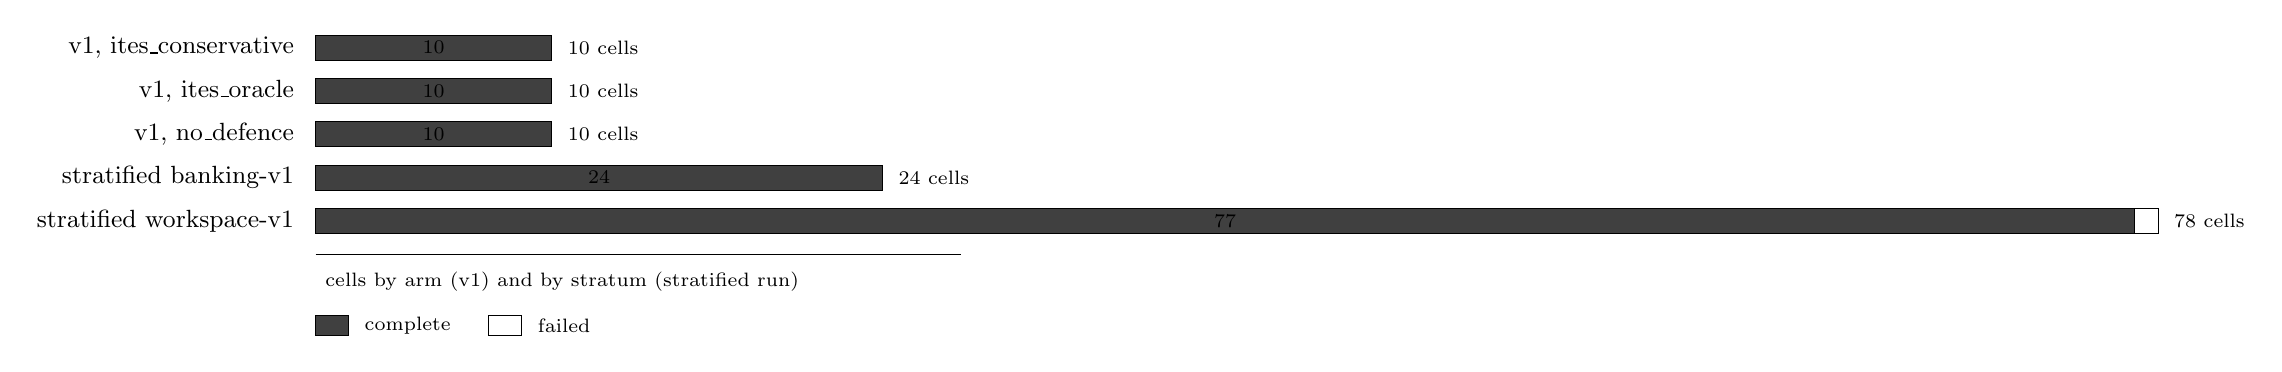
\begin{tikzpicture}[x=1cm,y=1cm]
  \node[anchor=east,font=\small] at (-0.15,0.16) {v1, ites\_conservative};
  \fill[black!75] (0.00,0.00) rectangle +(3.00,0.32);
  \draw[black,line width=0.3pt] (0.00,0.00) rectangle +(3.00,0.32);
  \node[font=\scriptsize] at (1.50,0.16) {10};
  \node[anchor=west,font=\scriptsize] at (3.08,0.16) {10 cells};
  \node[anchor=east,font=\small] at (-0.15,-0.39) {v1, ites\_oracle};
  \fill[black!75] (0.00,-0.55) rectangle +(3.00,0.32);
  \draw[black,line width=0.3pt] (0.00,-0.55) rectangle +(3.00,0.32);
  \node[font=\scriptsize] at (1.50,-0.39) {10};
  \node[anchor=west,font=\scriptsize] at (3.08,-0.39) {10 cells};
  \node[anchor=east,font=\small] at (-0.15,-0.94) {v1, no\_defence};
  \fill[black!75] (0.00,-1.10) rectangle +(3.00,0.32);
  \draw[black,line width=0.3pt] (0.00,-1.10) rectangle +(3.00,0.32);
  \node[font=\scriptsize] at (1.50,-0.94) {10};
  \node[anchor=west,font=\scriptsize] at (3.08,-0.94) {10 cells};
  \node[anchor=east,font=\small] at (-0.15,-1.49) {stratified banking-v1};
  \fill[black!75] (0.00,-1.65) rectangle +(7.20,0.32);
  \draw[black,line width=0.3pt] (0.00,-1.65) rectangle +(7.20,0.32);
  \node[font=\scriptsize] at (3.60,-1.49) {24};
  \node[anchor=west,font=\scriptsize] at (7.28,-1.49) {24 cells};
  \node[anchor=east,font=\small] at (-0.15,-2.04) {stratified workspace-v1};
  \fill[black!75] (0.00,-2.20) rectangle +(23.10,0.32);
  \draw[black,line width=0.3pt] (0.00,-2.20) rectangle +(23.10,0.32);
  \node[font=\scriptsize] at (11.55,-2.04) {77};
  \fill[white] (23.10,-2.20) rectangle +(0.30,0.32);
  \draw[black,line width=0.3pt] (23.10,-2.20) rectangle +(0.30,0.32);
  \node[anchor=west,font=\scriptsize] at (23.48,-2.04) {78 cells};
  \draw[black,line width=0.4pt] (0,-2.47) -- (8.2,-2.47);
  \node[anchor=north west,font=\scriptsize] at (0,-2.57) {cells by arm (v1) and by stratum (stratified run)};
  \fill[black!75] (0.0,-3.50) rectangle +(0.42,0.26);
  \draw[black,line width=0.3pt] (0.0,-3.50) rectangle +(0.42,0.26);
  \node[anchor=west,font=\scriptsize] at (0.50,-3.37) {complete};
  \fill[white] (2.2,-3.50) rectangle +(0.42,0.26);
  \draw[black,line width=0.3pt] (2.2,-3.50) rectangle +(0.42,0.26);
  \node[anchor=west,font=\scriptsize] at (2.70,-3.37) {failed};
\end{tikzpicture}
